\documentclass{standalone}
\usepackage{tikz}
\usetikzlibrary{patterns, positioning}
\usepackage[sfdefault]{ClearSans} %% option 'sfdefault' activates Clear Sans as the default text font
\usepackage[T1]{fontenc}

\begin{document}
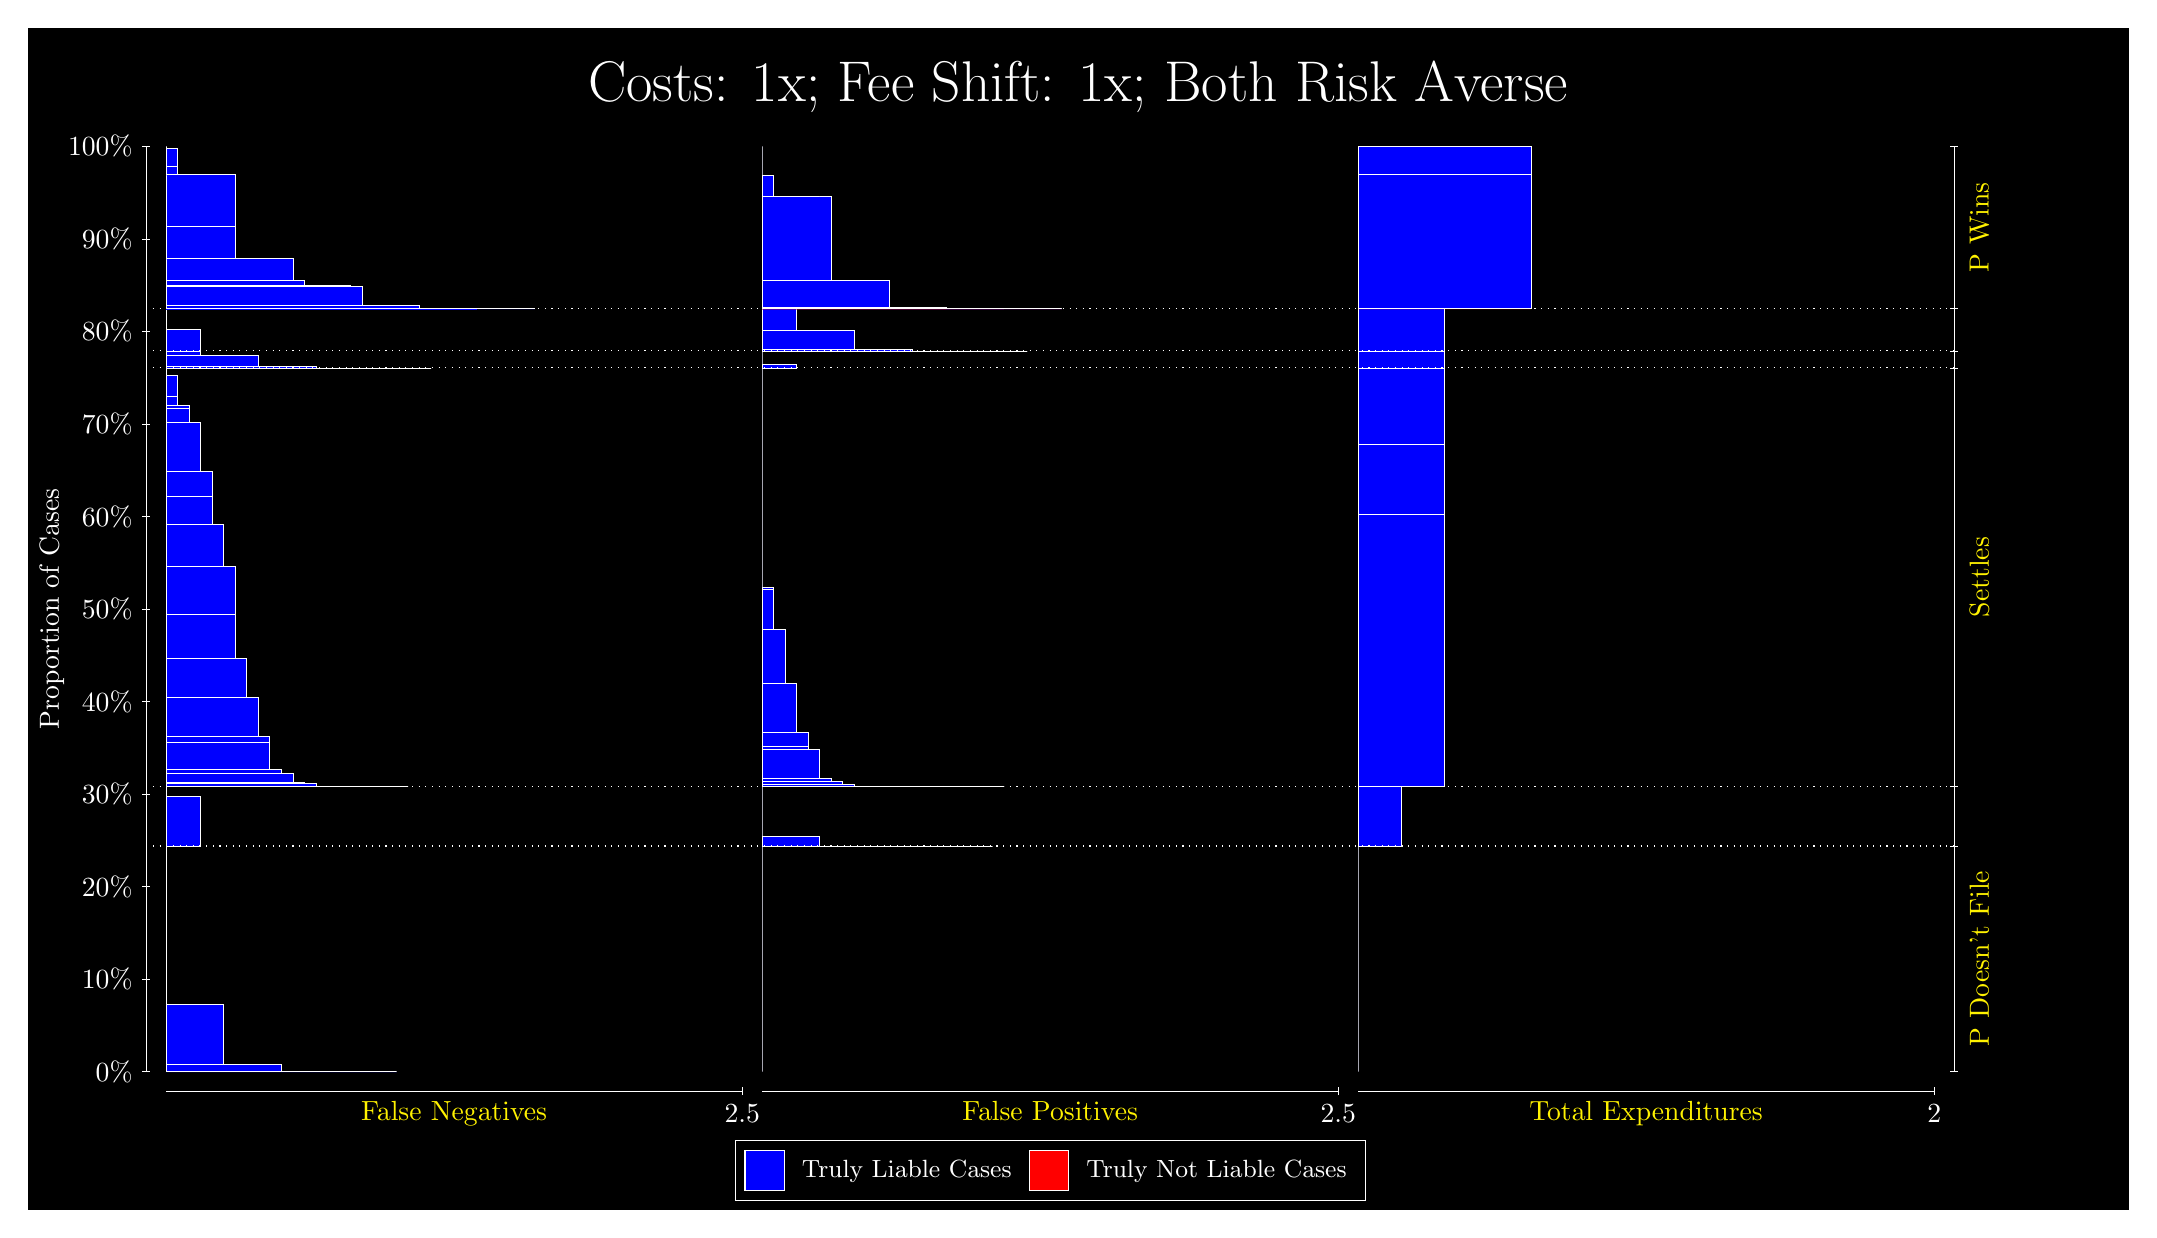
\begin{tikzpicture}
\draw[fill=black] (0,0) rectangle (26.667,15);
\draw[text=white] (0,13.5) rectangle (26.667,15) node[midway] {\huge Costs: 1x; Fee Shift: 1x; Both Risk Averse};
\draw[white, very thin] (1.5,1.75) -- (1.5,13.5);
\node[rotate=90, text=white, anchor=center] at (0.3, 7.625) {Proportion of Cases};
\draw[white, very thin] (1.45,1.75) -- (1.55,1.75);
\node[text=white, anchor=east] at (1.45, 1.75) {0\%};
\draw[white, very thin] (1.45,2.925) -- (1.55,2.925);
\node[text=white, anchor=east] at (1.45, 2.925) {10\%};
\draw[white, very thin] (1.45,4.1) -- (1.55,4.1);
\node[text=white, anchor=east] at (1.45, 4.1) {20\%};
\draw[white, very thin] (1.45,5.275) -- (1.55,5.275);
\node[text=white, anchor=east] at (1.45, 5.275) {30\%};
\draw[white, very thin] (1.45,6.45) -- (1.55,6.45);
\node[text=white, anchor=east] at (1.45, 6.45) {40\%};
\draw[white, very thin] (1.45,7.625) -- (1.55,7.625);
\node[text=white, anchor=east] at (1.45, 7.625) {50\%};
\draw[white, very thin] (1.45,8.8) -- (1.55,8.8);
\node[text=white, anchor=east] at (1.45, 8.8) {60\%};
\draw[white, very thin] (1.45,9.975) -- (1.55,9.975);
\node[text=white, anchor=east] at (1.45, 9.975) {70\%};
\draw[white, very thin] (1.45,11.15) -- (1.55,11.15);
\node[text=white, anchor=east] at (1.45, 11.15) {80\%};
\draw[white, very thin] (1.45,12.325) -- (1.55,12.325);
\node[text=white, anchor=east] at (1.45, 12.325) {90\%};
\draw[white, very thin] (1.45,13.5) -- (1.55,13.5);
\node[text=white, anchor=east] at (1.45, 13.5) {100\%};

\draw[white, very thin] (24.457,1.75) -- (24.457,13.5);
\draw[white, very thin] (24.407,1.75) -- (24.507,1.75);
\node[anchor=west] at (24.407, 1.75) {};
\draw[white, very thin] (24.407,4.6138) -- (24.507,4.6138);
\node[anchor=west] at (24.407, 4.6138) {};
\draw[white, very thin] (24.407,5.3738) -- (24.507,5.3738);
\node[anchor=west] at (24.407, 5.3738) {};
\draw[white, very thin] (24.407,10.687) -- (24.507,10.687);
\node[anchor=west] at (24.407, 10.687) {};
\draw[white, very thin] (24.407,10.903) -- (24.507,10.903);
\node[anchor=west] at (24.407, 10.903) {};
\draw[white, very thin] (24.407,11.437) -- (24.507,11.437);
\node[anchor=west] at (24.407, 11.437) {};
\draw[white, very thin] (24.407,13.5) -- (24.507,13.5);
\node[anchor=west] at (24.407, 13.5) {};

\draw[white, very thin, fill=blue] (1.75,1.75) rectangle (4.6775,1.75);
\draw[white, very thin, fill=blue] (1.75,1.75) rectangle (3.9457,1.7508);
\draw[white, very thin, fill=blue] (1.75,1.7508) rectangle (3.2138,1.8432);
\draw[white, very thin, fill=blue] (1.75,1.8432) rectangle (2.4819,2.6009);
\draw[white, very thin, fill=red] (1.75,2.6009) rectangle (1.75,2.6009);
\draw[white, very thin, fill=blue] (1.75,2.6009) rectangle (1.75,4.6138);
\draw[white, very thin, fill=blue] (1.75,4.6138) rectangle (2.1891,5.2494);
\draw[white, very thin, fill=red] (1.75,5.2494) rectangle (1.75,5.2494);
\draw[white, very thin, fill=blue] (1.75,5.2494) rectangle (1.75,5.3738);
\draw[white, very thin, fill=blue] (1.75,5.3738) rectangle (4.8239,5.3738);
\draw[white, very thin, fill=blue] (1.75,5.3738) rectangle (4.5312,5.3738);
\draw[white, very thin, fill=blue] (1.75,5.3738) rectangle (4.2384,5.3739);
\draw[white, very thin, fill=blue] (1.75,5.3739) rectangle (4.092,5.3739);
\draw[white, very thin, fill=blue] (1.75,5.3739) rectangle (3.9457,5.3741);
\draw[white, very thin, fill=blue] (1.75,5.3741) rectangle (3.7993,5.3743);
\draw[white, very thin, fill=blue] (1.75,5.3743) rectangle (3.6529,5.4092);
\draw[white, very thin, fill=blue] (1.75,5.4092) rectangle (3.5065,5.4238);
\draw[white, very thin, fill=blue] (1.75,5.4238) rectangle (3.3602,5.5424);
\draw[white, very thin, fill=blue] (1.75,5.5424) rectangle (3.2138,5.5935);
\draw[white, very thin, fill=blue] (1.75,5.5935) rectangle (3.0674,5.9258);
\draw[white, very thin, fill=blue] (1.75,5.9258) rectangle (3.0674,6.0049);
\draw[white, very thin, fill=blue] (1.75,6.0049) rectangle (2.921,6.5046);
\draw[white, very thin, fill=blue] (1.75,6.5046) rectangle (2.7746,6.9924);
\draw[white, very thin, fill=blue] (1.75,6.9924) rectangle (2.6283,7.5582);
\draw[white, very thin, fill=blue] (1.75,7.5582) rectangle (2.6283,8.1625);
\draw[white, very thin, fill=blue] (1.75,8.1625) rectangle (2.4819,8.6999);
\draw[white, very thin, fill=blue] (1.75,8.6999) rectangle (2.3355,9.0551);
\draw[white, very thin, fill=blue] (1.75,9.0551) rectangle (2.3355,9.3767);
\draw[white, very thin, fill=blue] (1.75,9.3767) rectangle (2.1891,10.001);
\draw[white, very thin, fill=blue] (1.75,10.001) rectangle (2.0428,10.179);
\draw[white, very thin, fill=blue] (1.75,10.179) rectangle (2.0428,10.213);
\draw[white, very thin, fill=blue] (1.75,10.213) rectangle (1.8964,10.326);
\draw[white, very thin, fill=blue] (1.75,10.326) rectangle (1.8964,10.586);
\draw[white, very thin, fill=blue] (1.75,10.586) rectangle (1.75,10.587);
\draw[white, very thin, fill=red] (1.75,10.587) rectangle (1.75,10.587);
\draw[white, very thin, fill=blue] (1.75,10.587) rectangle (1.75,10.687);
\draw[white, very thin, fill=blue] (1.75,10.687) rectangle (5.1167,10.687);
\draw[white, very thin, fill=blue] (1.75,10.687) rectangle (4.3848,10.687);
\draw[white, very thin, fill=blue] (1.75,10.687) rectangle (3.6529,10.705);
\draw[white, very thin, fill=blue] (1.75,10.705) rectangle (2.921,10.852);
\draw[white, very thin, fill=blue] (1.75,10.852) rectangle (2.1891,10.903);
\draw[white, very thin, fill=red] (1.75,10.903) rectangle (1.75,10.903);
\draw[white, very thin, fill=blue] (1.75,10.903) rectangle (2.1891,11.182);
\draw[white, very thin, fill=red] (1.75,11.182) rectangle (1.75,11.182);
\draw[white, very thin, fill=blue] (1.75,11.182) rectangle (1.75,11.437);
\draw[white, very thin, fill=blue] (1.75,11.437) rectangle (6.4341,11.437);
\draw[white, very thin, fill=blue] (1.75,11.437) rectangle (5.7022,11.438);
\draw[white, very thin, fill=blue] (1.75,11.438) rectangle (4.9703,11.477);
\draw[white, very thin, fill=blue] (1.75,11.477) rectangle (4.8239,11.477);
\draw[white, very thin, fill=blue] (1.75,11.477) rectangle (4.2384,11.728);
\draw[white, very thin, fill=blue] (1.75,11.728) rectangle (4.092,11.733);
\draw[white, very thin, fill=blue] (1.75,11.733) rectangle (3.5065,11.799);
\draw[white, very thin, fill=blue] (1.75,11.799) rectangle (3.3602,12.073);
\draw[white, very thin, fill=blue] (1.75,12.073) rectangle (2.7746,12.073);
\draw[white, very thin, fill=blue] (1.75,12.073) rectangle (2.6283,12.479);
\draw[white, very thin, fill=blue] (1.75,12.479) rectangle (2.6283,13.14);
\draw[white, very thin, fill=blue] (1.75,13.14) rectangle (2.0428,13.14);
\draw[white, very thin, fill=blue] (1.75,13.14) rectangle (1.8964,13.247);
\draw[white, very thin, fill=blue] (1.75,13.247) rectangle (1.8964,13.478);
\draw[white, very thin, fill=red] (1.75,13.478) rectangle (1.75,13.478);
\draw[white, very thin, fill=blue] (1.75,13.478) rectangle (1.75,13.5);
\draw[white, very thin, fill=red] (9.3189,1.75) rectangle (9.3189,1.75);
\draw[white, very thin, fill=blue] (9.3189,1.75) rectangle (9.3189,4.6138);
\draw[white, very thin, fill=red] (9.3189,4.6138) rectangle (12.246,4.6138);
\draw[white, very thin, fill=blue] (9.3189,4.6138) rectangle (12.246,4.6138);
\draw[white, very thin, fill=blue] (9.3189,4.6138) rectangle (11.515,4.6138);
\draw[white, very thin, fill=blue] (9.3189,4.6138) rectangle (10.783,4.6148);
\draw[white, very thin, fill=blue] (9.3189,4.6148) rectangle (10.051,4.7382);
\draw[white, very thin, fill=blue] (9.3189,4.7382) rectangle (9.3189,5.3738);
\draw[white, very thin, fill=red] (9.3189,5.3738) rectangle (12.393,5.3738);
\draw[white, very thin, fill=blue] (9.3189,5.3738) rectangle (12.393,5.3738);
\draw[white, very thin, fill=red] (9.3189,5.3738) rectangle (12.1,5.3738);
\draw[white, very thin, fill=blue] (9.3189,5.3738) rectangle (12.1,5.3738);
\draw[white, very thin, fill=red] (9.3189,5.3738) rectangle (11.807,5.3738);
\draw[white, very thin, fill=blue] (9.3189,5.3738) rectangle (11.807,5.3738);
\draw[white, very thin, fill=blue] (9.3189,5.3738) rectangle (11.661,5.3738);
\draw[white, very thin, fill=red] (9.3189,5.3738) rectangle (11.515,5.3738);
\draw[white, very thin, fill=blue] (9.3189,5.3738) rectangle (11.515,5.3738);
\draw[white, very thin, fill=blue] (9.3189,5.3738) rectangle (11.368,5.3738);
\draw[white, very thin, fill=red] (9.3189,5.3738) rectangle (11.222,5.3738);
\draw[white, very thin, fill=blue] (9.3189,5.3738) rectangle (11.222,5.3738);
\draw[white, very thin, fill=blue] (9.3189,5.3738) rectangle (11.075,5.3738);
\draw[white, very thin, fill=red] (9.3189,5.3738) rectangle (10.929,5.3738);
\draw[white, very thin, fill=blue] (9.3189,5.3738) rectangle (10.929,5.3739);
\draw[white, very thin, fill=red] (9.3189,5.3739) rectangle (10.929,5.3739);
\draw[white, very thin, fill=blue] (9.3189,5.3739) rectangle (10.929,5.3739);
\draw[white, very thin, fill=blue] (9.3189,5.3739) rectangle (10.783,5.3741);
\draw[white, very thin, fill=blue] (9.3189,5.3741) rectangle (10.636,5.3746);
\draw[white, very thin, fill=red] (9.3189,5.3746) rectangle (10.636,5.3746);
\draw[white, very thin, fill=blue] (9.3189,5.3746) rectangle (10.636,5.3771);
\draw[white, very thin, fill=blue] (9.3189,5.3771) rectangle (10.49,5.4011);
\draw[white, very thin, fill=red] (9.3189,5.4011) rectangle (10.344,5.4011);
\draw[white, very thin, fill=blue] (9.3189,5.4011) rectangle (10.344,5.4372);
\draw[white, very thin, fill=blue] (9.3189,5.4372) rectangle (10.197,5.474);
\draw[white, very thin, fill=blue] (9.3189,5.474) rectangle (10.197,5.4748);
\draw[white, very thin, fill=red] (9.3189,5.4748) rectangle (10.051,5.4748);
\draw[white, very thin, fill=blue] (9.3189,5.4748) rectangle (10.051,5.8482);
\draw[white, very thin, fill=blue] (9.3189,5.8482) rectangle (9.9044,5.8817);
\draw[white, very thin, fill=blue] (9.3189,5.8817) rectangle (9.9044,6.0604);
\draw[white, very thin, fill=blue] (9.3189,6.0604) rectangle (9.758,6.6843);
\draw[white, very thin, fill=blue] (9.3189,6.6843) rectangle (9.6116,7.3611);
\draw[white, very thin, fill=blue] (9.3189,7.3611) rectangle (9.4652,7.8771);
\draw[white, very thin, fill=blue] (9.3189,7.8771) rectangle (9.4652,7.8986);
\draw[white, very thin, fill=blue] (9.3189,7.8986) rectangle (9.3189,10.687);
\draw[white, very thin, fill=red] (9.3189,10.687) rectangle (9.758,10.687);
\draw[white, very thin, fill=blue] (9.3189,10.687) rectangle (9.758,10.738);
\draw[white, very thin, fill=blue] (9.3189,10.738) rectangle (9.3189,10.903);
\draw[white, very thin, fill=red] (9.3189,10.903) rectangle (12.686,10.903);
\draw[white, very thin, fill=blue] (9.3189,10.903) rectangle (12.686,10.903);
\draw[white, very thin, fill=blue] (9.3189,10.903) rectangle (11.954,10.903);
\draw[white, very thin, fill=blue] (9.3189,10.903) rectangle (11.222,10.922);
\draw[white, very thin, fill=blue] (9.3189,10.922) rectangle (10.49,11.158);
\draw[white, very thin, fill=blue] (9.3189,11.158) rectangle (9.758,11.437);
\draw[white, very thin, fill=red] (9.3189,11.437) rectangle (13.125,11.437);
\draw[white, very thin, fill=blue] (9.3189,11.437) rectangle (13.125,11.437);
\draw[white, very thin, fill=red] (9.3189,11.437) rectangle (12.393,11.437);
\draw[white, very thin, fill=blue] (9.3189,11.437) rectangle (12.393,11.437);
\draw[white, very thin, fill=red] (9.3189,11.437) rectangle (11.661,11.437);
\draw[white, very thin, fill=blue] (9.3189,11.437) rectangle (11.661,11.46);
\draw[white, very thin, fill=red] (9.3189,11.46) rectangle (10.929,11.46);
\draw[white, very thin, fill=blue] (9.3189,11.46) rectangle (10.929,11.797);
\draw[white, very thin, fill=red] (9.3189,11.797) rectangle (10.783,11.797);
\draw[white, very thin, fill=blue] (9.3189,11.797) rectangle (10.783,11.797);
\draw[white, very thin, fill=blue] (9.3189,11.797) rectangle (10.197,12.864);
\draw[white, very thin, fill=red] (9.3189,12.864) rectangle (10.051,12.864);
\draw[white, very thin, fill=blue] (9.3189,12.864) rectangle (10.051,12.864);
\draw[white, very thin, fill=blue] (9.3189,12.864) rectangle (9.4652,13.138);
\draw[white, very thin, fill=red] (9.3189,13.138) rectangle (9.3189,13.138);
\draw[white, very thin, fill=blue] (9.3189,13.138) rectangle (9.3189,13.5);
\draw[white, very thin, fill=red] (16.888,1.75) rectangle (16.888,1.75);
\draw[white, very thin, fill=blue] (16.888,1.75) rectangle (16.888,4.6138);
\draw[white, very thin, fill=red] (16.888,4.6138) rectangle (17.437,4.6138);
\draw[white, very thin, fill=blue] (16.888,4.6138) rectangle (17.437,5.3738);
\draw[white, very thin, fill=red] (16.888,5.3738) rectangle (17.986,5.3738);
\draw[white, very thin, fill=blue] (16.888,5.3738) rectangle (17.986,8.8254);
\draw[white, very thin, fill=red] (16.888,8.8254) rectangle (17.986,8.8254);
\draw[white, very thin, fill=blue] (16.888,8.8254) rectangle (17.986,9.7149);
\draw[white, very thin, fill=red] (16.888,9.7149) rectangle (17.986,9.7149);
\draw[white, very thin, fill=blue] (16.888,9.7149) rectangle (17.986,10.687);
\draw[white, very thin, fill=red] (16.888,10.687) rectangle (17.986,10.687);
\draw[white, very thin, fill=blue] (16.888,10.687) rectangle (17.986,10.903);
\draw[white, very thin, fill=red] (16.888,10.903) rectangle (17.986,10.903);
\draw[white, very thin, fill=blue] (16.888,10.903) rectangle (17.986,11.437);
\draw[white, very thin, fill=red] (16.888,11.437) rectangle (19.083,11.437);
\draw[white, very thin, fill=blue] (16.888,11.437) rectangle (19.083,13.143);
\draw[white, very thin, fill=red] (16.888,13.143) rectangle (19.083,13.143);
\draw[white, very thin, fill=blue] (16.888,13.143) rectangle (19.083,13.5);
\draw[white, dotted] (1.5,4.6138) -- (24.457,4.6138);
\draw[white, dotted] (1.5,5.3738) -- (24.457,5.3738);
\draw[white, dotted] (1.5,10.687) -- (24.457,10.687);
\draw[white, dotted] (1.5,10.903) -- (24.457,10.903);
\draw[white, dotted] (1.5,11.437) -- (24.457,11.437);
\draw[white, very thin] (1.75,1.5) -- (9.0689,1.5);
\node[text=yellow, anchor=north] at (5.4094, 1.5) {False Negatives};
\draw[white, very thin] (9.0689,1.45) -- (9.0689,1.55);
\node[text=white, anchor=north] at (9.0689, 1.45) {2.5};

\draw[white, very thin] (9.3189,1.5) -- (16.638,1.5);
\node[text=yellow, anchor=north] at (12.978, 1.5) {False Positives};
\draw[white, very thin] (16.638,1.45) -- (16.638,1.55);
\node[text=white, anchor=north] at (16.638, 1.45) {2.5};

\draw[white, very thin] (16.888,1.5) -- (24.207,1.5);
\node[text=yellow, anchor=north] at (20.547, 1.5) {Total Expenditures};
\draw[white, very thin] (24.207,1.45) -- (24.207,1.55);
\node[text=white, anchor=north] at (24.207, 1.45) {2};

\node[text=yellow, centered, rotate=90] at (24.777, 3.1819) {P Doesn't File};

\node[text=yellow, centered, rotate=90] at (24.777, 8.0305) {Settles};


\node[text=yellow, centered, rotate=90] at (24.777, 12.469) {P Wins};

\draw (12.978300999999998,1.5) node[draw=none] (baseCoordinate) {};
\begin{scope}[align=center]
        \matrix[scale=0.5, draw=white, below=0.5cm of baseCoordinate, nodes={draw}, column sep=0.1cm]{
            \node[rectangle, draw, minimum width=0.5cm, minimum height=0.5cm, fill=blue] {}; &
            \node[draw=none, font=\small, text=white] (B) {Truly Liable Cases}; &
            \node[rectangle, draw, minimum width=0.5cm, minimum height=0.5cm, fill=red] {}; &
            \node[draw=none, font=\small, text=white] (B) {Truly Not Liable Cases}; \\
            };
\end{scope}

\end{tikzpicture}
\end{document}